\documentclass[book.tex]{subfiles}
\begin{document}

if Software was funded during February 1991 by four people: 

 \begin{figure}[H]
\centering  
\begin{tabular}{ l  c  l}
  \toprule
  \textbf{Name} &  \textbf{Age} & \textbf{Occupation} \\
  \toprule 
   John Carmack & 22 &  Technical Director\\
   John Romero & 25 &  Level Artist\\
   Adrian Carmack & 22 &  Artist\\
   Tom Hall & 28 &  Game Designer\\
     \toprule
\end{tabular}
\caption{id Software founding members.}\label{fig:Id Software team}
\end{figure}

Wolfenstein 3D would be the first title for id but the team had already shipped no less than 13 games will working for their previous employer SoftDisk:\\
\begin{itemize}
  \item Dangerous Dave (1988)\footnote{Dangerous Dave is a solo project of John Romero predating Id's formation, but Id Software produced its first sequel and it is sometimes regarded as an early Id Software title. Later Dangerous Dave sequels were not made by Id, nor were later Catacomb titles.}
  \item Commander Keen
  \begin{itemize}
    \item Episode 1: Marooned on Mars (1990)
    \item Episode 2: The Earth Explodes (1991)
    \item Episode 3: Keen Must Die (1991)
    \item Keen Dreams (1991)
    \item Episode 4: Secret of the Oracle (1991)
    \item Episode 5: The Armageddon Machine (1991)
    \item Episode 6: Aliens Ate My Baby Sitter (1991)
  \end{itemize}
  
  \item Dangerous Dave in the Haunted Mansion (1991)
  \item Rescue Rover (1991)
  \item Rescue Rover 2 (1991)
  \item Shadow Knights (1991)
  \item Hovertank 3D (1991)
  \item Catacomb 3D: A New Dimension (1991)
\end{itemize}


Considering the magnitude and ambitions of the title, four more people were added to the team for a total of eight people.\\

 \begin{figure}[H]
\centering  
\begin{tabular}{ l  c  l}
  \toprule
  \textbf{Name} &  \textbf{Age} & \textbf{Occupation} \\
  \toprule 
   Jay Wilbur & ?? &  Business\\
   Kevin Cloud & 27 &  Computer Artist\\
   Robert Prince & ?? &  Composer\\
   Jason Blochowiak & ?? &  Additional Programming\\
     \toprule
\end{tabular}
\caption{id Software new hires.}\label{fig:Id Software hires}
\end{figure}

Every member was working with an high end 386 DX. As for combining game, tools and assets:\\

 \begin{fancyquotes}
We started with floppy data transfer, but we had a Novell network on coax Ethernet by the end. We didn't have a version control system.  Surprisingly, we went all the way to Quake 3 without one, then we started using Visual Source Safe.\\
 \\
\textbf{John Carmack - Programmer}
\end{fancyquotes}
\section{Programming}

\begin{fancyquotes}
At that point, we wanted 21" monitors, but couldn't justify them.  I used a second mono monitor to allow Turbo Debugger 386 to keep the main screen in graphics mode while I stepped through the code.
 \\
\textbf{John Carmack - Programmer}
\end{fancyquotes}




\begin{fancyquotes}
Jason was part of Id at the start, but we parted ways during Wolf development.
 \bigskip \\
\textbf{John Carmack - Programmer}
 \end{fancyquotes}
 
 
 
\section{Graphics assets}
Deluxe Paint\\

\begin{fancyquotes}
Yep, we didn't have any scanning tools at the time.\\
\\
\textbf{John Carmack - Programmer}
\end{fancyquotes}
\section{Programming}
	
\begin{figure}[H]
\centering
 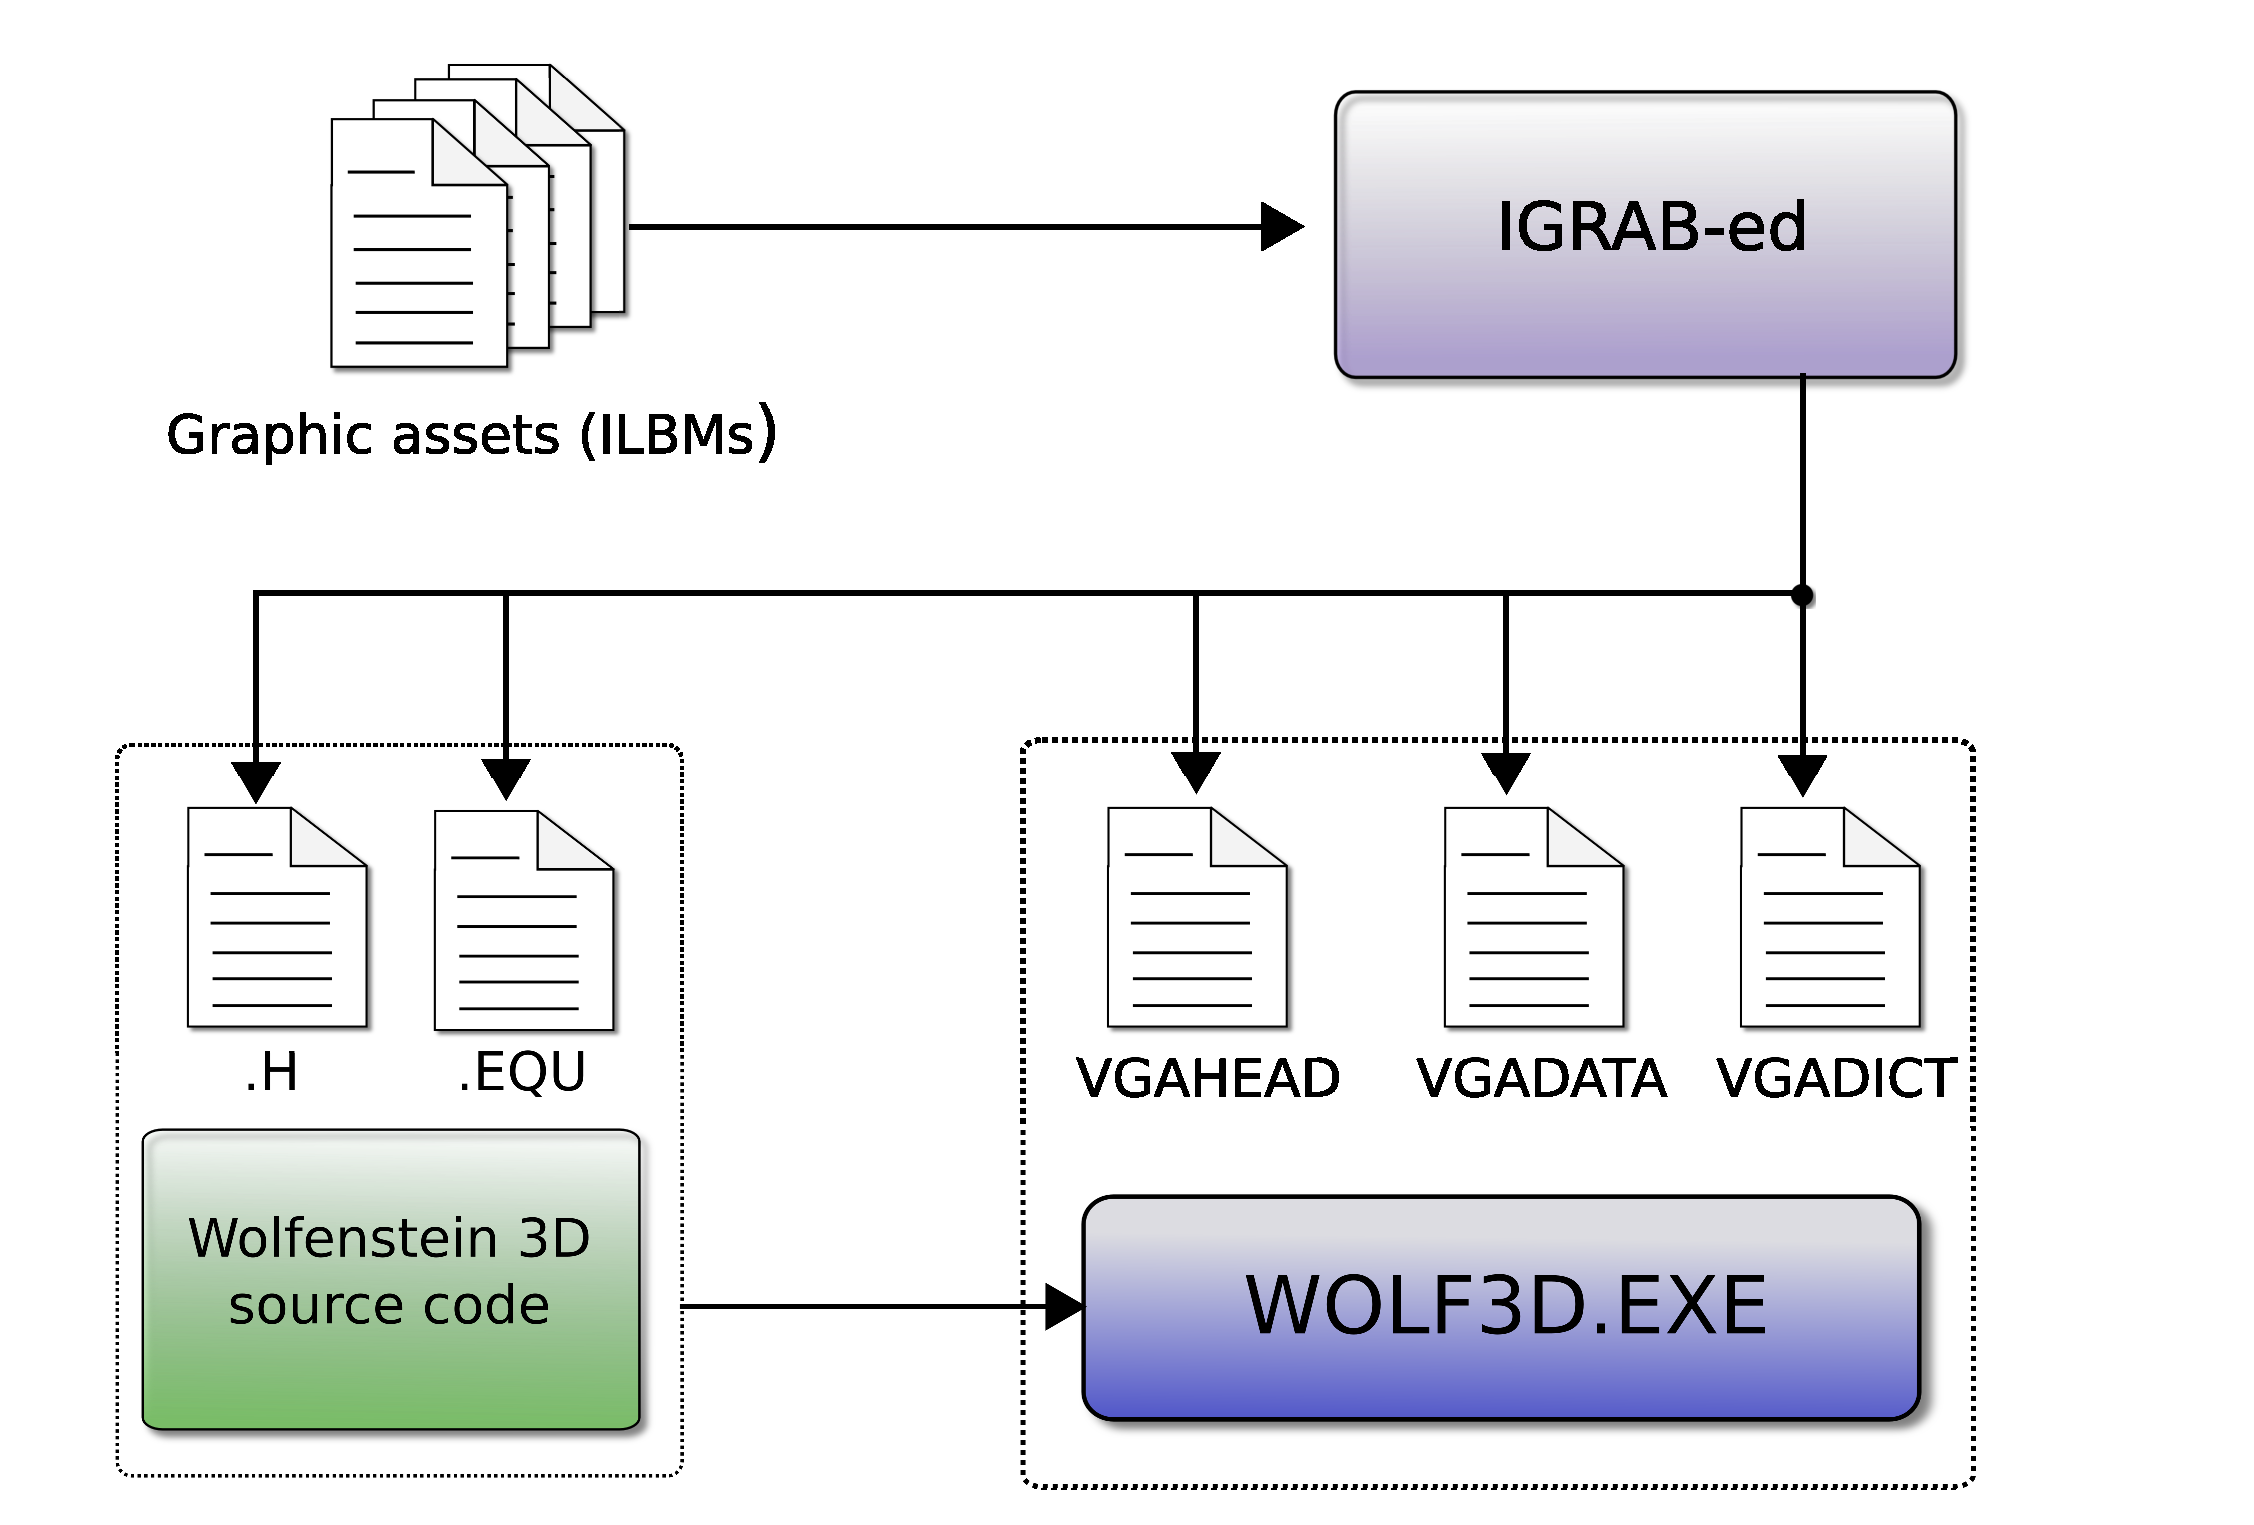
\includegraphics[scale=0.4]{imgs/drawing_plain.eps}
 \caption{Integer layout.} \label{fig:mips}
 \end{figure}

\section{Maps}
\section{Business}
\section{Sounds}
\section{Distribution}
	\subsection{Compression}
	\subsection{Shareware model}
\end{document}




